%%%%%%%%%%%%%%%%%%%%%%%%%%%%%%%%%%%%%%%%%%%%%%%%%%%%%%%%%%%%%%%%%%%%%%%%%%%
%
% Template for a LaTex article in English.
%
%%%%%%%%%%%%%%%%%%%%%%%%%%%%%%%%%%%%%%%%%%%%%%%%%%%%%%%%%%%%%%%%%%%%%%%%%%%

\documentclass{article}

% AMS packages:
\usepackage{amsmath, amsthm, amsfonts}
\usepackage{algorithm}
\usepackage[hyperref, UTF8]{ctex}
\usepackage[noend]{algpseudocode}
\usepackage{graphicx}
\usepackage{subcaption}
\graphicspath{ {images/} }

% Theorems
%-----------------------------------------------------------------
\newtheorem{thm}{Theorem}[section]
\newtheorem{cor}[thm]{Corollary}
\newtheorem{lem}[thm]{Lemma}
\newtheorem{prop}[thm]{Proposition}
\theoremstyle{definition}
\newtheorem{defn}[thm]{Definition}
\theoremstyle{remark}
\newtheorem{rem}[thm]{Remark}

\makeatletter
\def\BState{\State\hskip-\ALG@thistlm}
\makeatother
%\newcommand*{\rom}[1]{\expandafter\@slowromancap\romannumeral #1@}
\newcommand{\rom}[1]{\uppercase\expandafter{\romannumeral #1\relax}}
% Shortcuts.
% One can define new commands to shorten frequently used
% constructions. As an example, this defines the R and Z used
% for the real and integer numbers.
%-----------------------------------------------------------------
\def\RR{\mathbb{R}}
\def\ZZ{\mathbb{Z}}

% Similarly, one can define commands that take arguments. In this
% example we define a command for the absolute value.
% -----------------------------------------------------------------
\newcommand{\abs}[1]{\left\vert#1\right\vert}

% Operators
% New operators must defined as such to have them typeset
% correctly. As an example we define the Jacobian:
% -----------------------------------------------------------------
\DeclareMathOperator{\Jac}{Jac}

%-----------------------------------------------------------------
\title{Work Report}
\author{ShengweiZHANG\\
  %% \small Dept. Templates and Editors\\
  %% \small E12345\\
  %% \small Spain
}

\begin{document}
\maketitle

%% \abstract{Compiling Embedded\_thin\_shell progress}
\section{6.15-6.19工作}
\begin{itemize}
	\item 将code中的mesh表示转为opepnmesh
        \item 将翻边加入到双边滤波器
	\item 尝试通过动态调整邻域大小(法向变化小的区域选取大的邻域,而在法向变化大的区域使用小的邻域)来smooth模型.
\end{itemize}
\section{结果与分析}
\subsection{策略1}
一环邻域的两种选取方法:
\begin{itemize}
  \item $N_I(i)$ , 与面片i共享边的面片
  \item $N_{II}(i)$, 与面片i共享顶点的面片
\end{itemize}
根据上一个报告,由于$N_{II}$比$N_{I}$扩大了邻域得到的结果往往更光滑(去噪效果更好),而在边界处会使法向更快地收敛(产生锐利的棱角,不是我们所期望的)。\par
所以我使用$N_{II}$滤波,迭代8次,对于任意的一个面片i和其一环邻域 如果$max(normal(i) \cdot normal(j)) < cos(\pi/6), j \in N_{II}(i)$,那么该面片使用$N_{II}$,否则就使用$N_I$, 对原模型从新做滤波.
\subsection{策略2}
根据Atos中的几个滤波选项:
\begin{itemize}
  \item  Filter radius, states how large the environment is which is considered for each polygon point.
  \item Detail sharpness determines how well details of the measuring object are maintained. The function limits the filter radius at object details and edges.
  \item Surface tolerance, determines the maximum roughness(noise) which you want to thin. The software thins only those areas of the mesh for which the roughness is smaller than the specified value.
\end{itemize}
据此,我用$N_I$的测地距离来圈定邻域并给双边滤波器加入三个额外参数:
\begin{itemize}
  \item $r_{min}$ 最小滤波半径 $r_{ij} < r_{min}, j\in N_{i}$ 
  \item ${r_{max}}$ 最大滤波半径 $r_{ij} > r_{max}, j \notin N_{i}$ 
  \item $\theta$  对于测地距离$r_{max}>r_{ij} >r_{min}$ 如果 $normal(i) \cdot normal(j) > cos(\theta)$ 则面片 $j\in N_{i}$
 \end{itemize}
\subsection{结果对比与分析}
\begin{figure}[H]
  	\begin{subfigure}[b]{0.5\textwidth}
        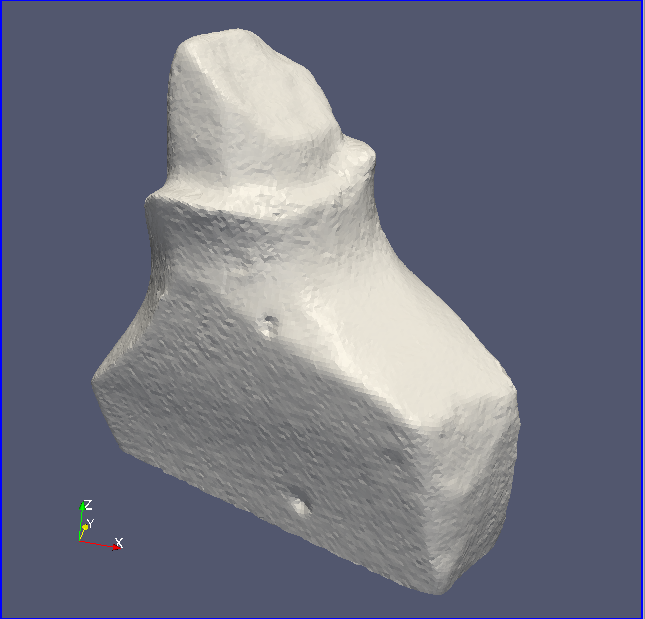
\includegraphics[width=\textwidth]{input_1}
        \caption[input]{输入模型}
        \end{subfigure}
        \begin{subfigure}[b]{0.5\textwidth}
        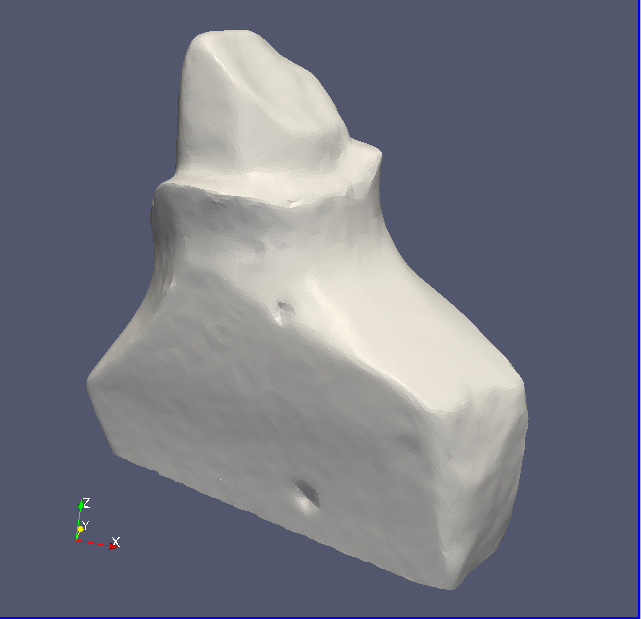
\includegraphics[width=\textwidth]{basic_1}
        \caption[basic]{标准双边滤波器结果}
        \end{subfigure}
        \begin{subfigure}[b]{0.5\textwidth}
        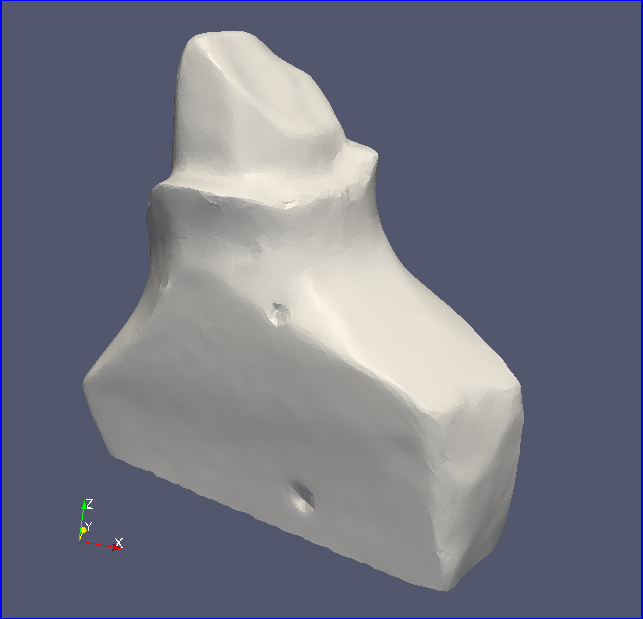
\includegraphics[width=\textwidth]{v2_1}
        \caption[our]{方案2结果}
        \end{subfigure}
        \begin{subfigure}[b]{0.5\textwidth}
	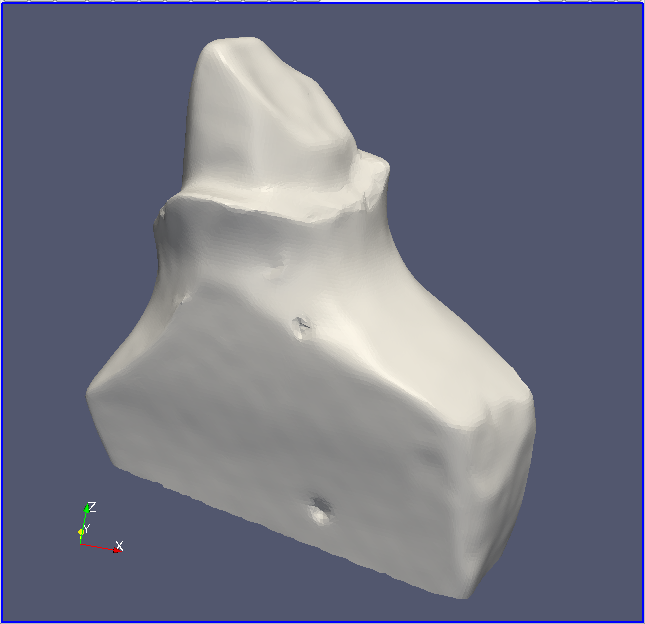
\includegraphics[width=\textwidth]{atos_1}
        \caption[atos]{Atos结果}
        \end{subfigure}
        \caption[不同方法滤波效果对比]
	{不同方法滤波效果对比1}
\end{figure}
\begin{figure}[H]
  	\begin{subfigure}[b]{0.5\textwidth}
        \includegraphics[width=\textwidth]{input_2}
        \caption[input]{输入模型}
        \end{subfigure}
        \begin{subfigure}[b]{0.5\textwidth}
        \includegraphics[width=\textwidth]{basic_2}
        \caption[basic]{标准双边滤波器结果}
        \end{subfigure}
        \begin{subfigure}[b]{0.5\textwidth}
        \includegraphics[width=\textwidth]{v2_2}
        \caption[our]{方案2结果}
        \end{subfigure}
        \begin{subfigure}[b]{0.5\textwidth}
	\includegraphics[width=\textwidth]{atos_2}
        \caption[atos]{Atos结果}
        \end{subfigure}
        \caption[不同方法滤波效果对比]
	{不同方法滤波效果对比2}
\end{figure}
\end{document}
